\documentclass[11pt]{article}
\usepackage[margin=1in]{geometry}
\usepackage{booktabs}
\usepackage{graphicx}
\usepackage{tabularx}
\usepackage{float}
\usepackage{hyperref}
\usepackage{enumitem}
\usepackage{longtable}
\usepackage{array}
\hypersetup{colorlinks=true, linkcolor=blue, urlcolor=blue}
\setlength{\parindent}{0pt}
\setlength{\parskip}{0.6em}

\title{Cross-Dataset Rollout Statistics Report for Qwen/Qwen3-1.7B}
\author{Murphy}
\date{2026-03-14T19:26:23.196702+00:00}

\begin{document}
\maketitle

\section*{Scope}
This report consolidates the full math $\rightarrow$ GPQA $\rightarrow$ MMLU-Pro $\rightarrow$ LiveCodeBench rollout-stat sweep for \texttt{Qwen/Qwen3-1.7B}. The collector uses the n-gram loop detector with \texttt{n=30} and \texttt{k=20} and records both top-level event rates and overlap statistics between looping, max-model-length termination, and correctness.

The math block was evaluated as two separate datasets under the same freeform prompt contract: \texttt{MATH-500} (500 samples) and \texttt{AIME 2024/2025} (60 samples). The downstream multiple-choice and code-generation blocks were evaluated on \texttt{GPQA Diamond}, \texttt{MMLU-Pro}, and \texttt{LiveCodeBench release\_v6} in the same rollout pipeline.

\section*{Datasets and Prompt Formats}
\paragraph{MATH-500}
\textbf{Task kind.} \texttt{math\_freeform}
\textbf{Dataset.} 500 free-form math problems from the HuggingFaceH4 MATH-500 test split.
\textbf{Chat / prompt format.} Tokenizer chat template with one user turn: the raw problem text followed by 'You must put your final answer within \textbackslash{}\textbackslash{}boxed\{\}.'

\paragraph{AIME 2024/2025}
\textbf{Task kind.} \texttt{math\_freeform}
\textbf{Dataset.} A local 60-row JSONL made by concatenating the AIME 2024 and 2025 test splits into question/answer records.
\textbf{Chat / prompt format.} The same math-freeform Qwen chat template as MATH-500: one user turn with the problem plus a final-answer-in-box instruction.

\paragraph{GPQA Diamond}
\textbf{Task kind.} \texttt{multiple\_choice\_gpqa}
\textbf{Dataset.} A local staged GPQA Diamond CSV with 198 graduate-level science questions and shuffled four-way answer options.
\textbf{Chat / prompt format.} Tokenizer chat template with one user turn containing the question, a shuffled A-D answer block, and the instruction to respond with a single best answer letter.

\paragraph{MMLU-Pro}
\textbf{Task kind.} \texttt{multiple\_choice\_mmlupro}
\textbf{Dataset.} The TIGER-Lab MMLU-Pro test split, capped to 2000 examples for this rollout pass. Requested cap: at most 2000 samples.
\textbf{Chat / prompt format.} Tokenizer chat template with one user turn containing the question, an A-J answer list, and the instruction to return only the best answer letter.

\paragraph{LiveCodeBench release\_v6}
\textbf{Task kind.} \texttt{livecodebench\_codegen}
\textbf{Dataset.} 1055 LiveCodeBench code-generation problems formed by concatenating test.jsonl through test6.jsonl and sorting by question\_id.
\textbf{Chat / prompt format.} LiveCodeBench's format\_prompt\_generation pipeline with LM style CodeQwenInstruct, producing raw string prompts rather than a tokenizer chat-template wrapper.

\section*{Generation Configuration}
The common collector configuration across all runs is:
\begin{itemize}[leftmargin=1.5em]
\item Model: \texttt{Qwen/Qwen3-1.7B}
\item Seed: \texttt{0}
\item Loop detector: \texttt{n=30, k=20}
\item Common settings shared by every dataset JSON: \texttt{temperature=0.0}, \texttt{dtype=bfloat16}, and \texttt{trust\_remote\_code=True}
\end{itemize}

Per-dataset runtime settings are:
\begin{tabular}{lrrrrrrr}
\toprule
Dataset & Temp & Max tokens & Max model len & TP & DP & Max seqs & Batch toks \\
\midrule
MATH-500 & 0.0 & 81920 & 40960 & 1 & 4 & 8 & 4096 \\
AIME 2024/2025 & 0.0 & 81920 & 40960 & 1 & 4 & 8 & 4096 \\
GPQA Diamond & 0.0 & 81920 & 40960 & 1 & 1 & 16 & NA \\
MMLU-Pro & 0.0 & 81920 & 40960 & 1 & 3 & 8 & 4096 \\
LiveCodeBench release\_v6 & 0.0 & 81920 & 40960 & 1 & 4 & 8 & 4096 \\
\bottomrule
\end{tabular}

\section*{Statistics Logged}
The refreshed collector contract tracks the following metrics across the bundle (13 named metrics in the union):
\begin{itemize}[leftmargin=1.5em]
\item \texttt{avg\_correct\_generation\_length}: Average generated length restricted to correct rollouts.
\item \texttt{avg\_first\_loop\_prefix\_length}: Average prefix length before the first detected loop.
\item \texttt{avg\_generation\_length}: Average number of generated tokens per rollout.
\item \texttt{avg\_loop\_generation\_length}: Average generated length restricted to looped rollouts.
\item \texttt{avg\_wrong\_generation\_length}: Average generated length restricted to wrong rollouts.
\item \texttt{generation\_length\_variance}: Variance of generated token counts across graded rollouts.
\item \texttt{loop\_fraction}: Fraction of graded rollouts flagged by the n-gram loop detector.
\item \texttt{loop\_max\_length\_hit\_fraction}: Among looped rollouts, fraction that also hit max model length.
\item \texttt{loop\_success\_fraction}: Among looped rollouts, fraction that were still correct.
\item \texttt{max\_length\_hit\_fraction}: Fraction of rollouts that terminated at the model-length limit.
\item \texttt{max\_length\_hit\_loop\_fraction}: Among max-length-hit rollouts, fraction that were also looped.
\item \texttt{max\_length\_hit\_success\_fraction}: Among max-length-hit rollouts, fraction that were correct.
\item \texttt{success\_fraction}: Fraction of graded rollouts with the correct answer.
\end{itemize}

The JSON payloads also retain the raw event counts for samples, correct vs. wrong rollouts, looped rollouts, max-length hits, and their pairwise intersections.

\section*{Results Summary}
\begin{tabular}{lrrrrrr}
\toprule
Dataset & Samples & Correct & Looped & Max length & Loop+Max & Loop+Correct \\
\midrule
MATH-500 & 500 & 72.0\% & 4.2\% & 2.2\% & 52.4\% & 28.6\% \\
AIME 2024/2025 & 60 & 36.7\% & 16.7\% & 15.0\% & 90.0\% & 10.0\% \\
GPQA Diamond & 198 & 37.4\% & 31.3\% & 20.2\% & 64.5\% & 27.4\% \\
MMLU-Pro & 2000 & 42.9\% & 6.9\% & 3.0\% & 44.2\% & 22.5\% \\
LiveCodeBench release\_v6 & 1055 & 49.3\% & 25.3\% & 20.9\% & 82.0\% & 3.4\% \\
\bottomrule
\end{tabular}

\begin{itemize}[leftmargin=1.5em]
\item MATH-500: correct 360/500 (72.0\%); looped 21/500 (4.2\%); max-length hits 11/500 (2.2\%); looped and max-length 11/21 (52.4\%); max-length and looped 11/11 (100.0\%); looped and correct 6/21 (28.6\%).
\item AIME 2024/2025: correct 22/60 (36.7\%); looped 10/60 (16.7\%); max-length hits 9/60 (15.0\%); looped and max-length 9/10 (90.0\%); max-length and looped 9/9 (100.0\%); looped and correct 1/10 (10.0\%).
\item GPQA Diamond: correct 74/198 (37.4\%); looped 62/198 (31.3\%); max-length hits 40/198 (20.2\%); looped and max-length 40/62 (64.5\%); max-length and looped 40/40 (100.0\%); looped and correct 17/62 (27.4\%).
\item MMLU-Pro: correct 857/2000 (42.9\%); looped 138/2000 (6.9\%); max-length hits 61/2000 (3.0\%); looped and max-length 61/138 (44.2\%); max-length and looped 61/61 (100.0\%); looped and correct 31/138 (22.5\%).
\item LiveCodeBench release\_v6: correct 520/1055 (49.3\%); looped 267/1055 (25.3\%); max-length hits 220/1055 (20.9\%); looped and max-length 219/267 (82.0\%); max-length and looped 219/220 (99.5\%); looped and correct 9/267 (3.4\%).
\end{itemize}

\subsection*{Headline observations}
The largest raw loop rate appears on GPQA Diamond at 31.3\%, while MATH-500 is the most stable dataset in this bundle at 4.2\%.
The longest looped generations also appear on AIME 2024/2025: 38641.5 tokens on average, with the first detected loop not appearing until 11782.3 tokens.
Max-length termination is almost synonymous with looping on the hardest long-form settings: MATH-500 reaches 100.0\% for the max-length-hit loop conditional.
The most forgiving loop regime is MATH-500, where 28.6\% of looped rollouts still end in a correct answer.

\begin{figure}[H]
\centering
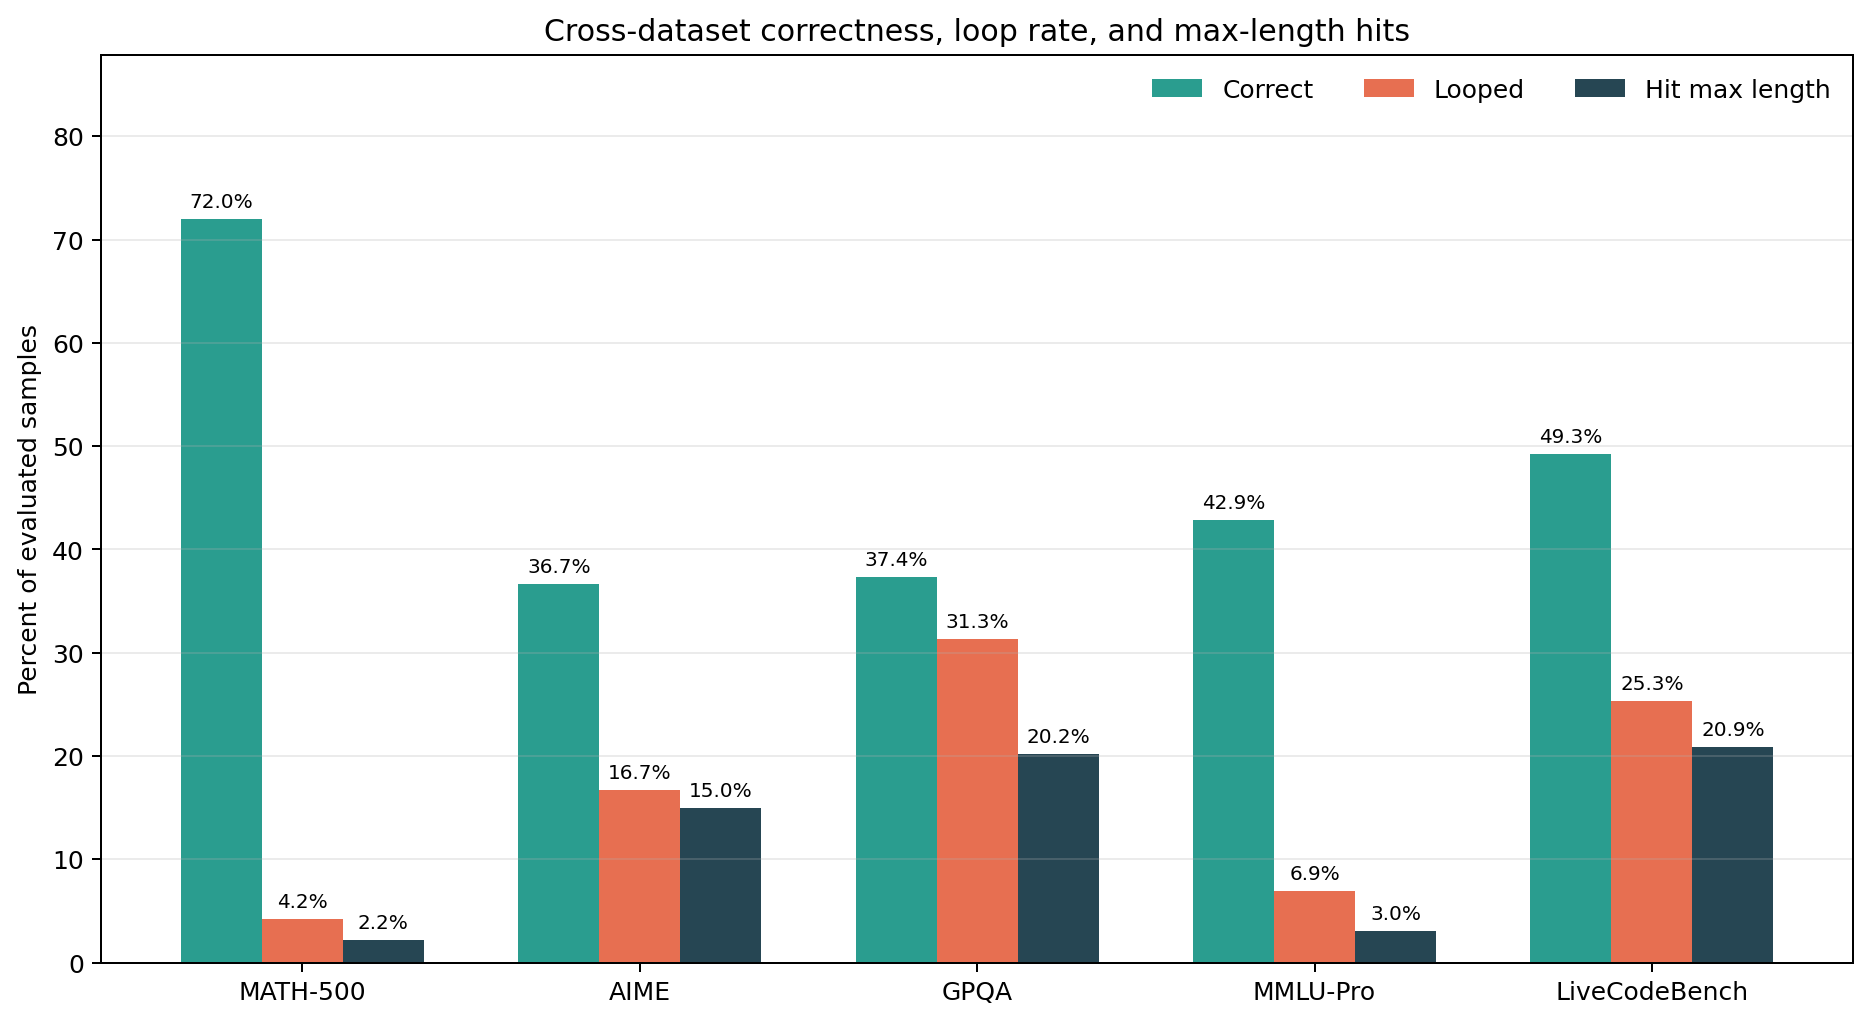
\includegraphics[width=\textwidth]{figures/cross_dataset_rates.png}
\caption{Correctness, loop rate, and max-length-hit rate for each evaluated dataset.}
\end{figure}

\begin{figure}[H]
\centering
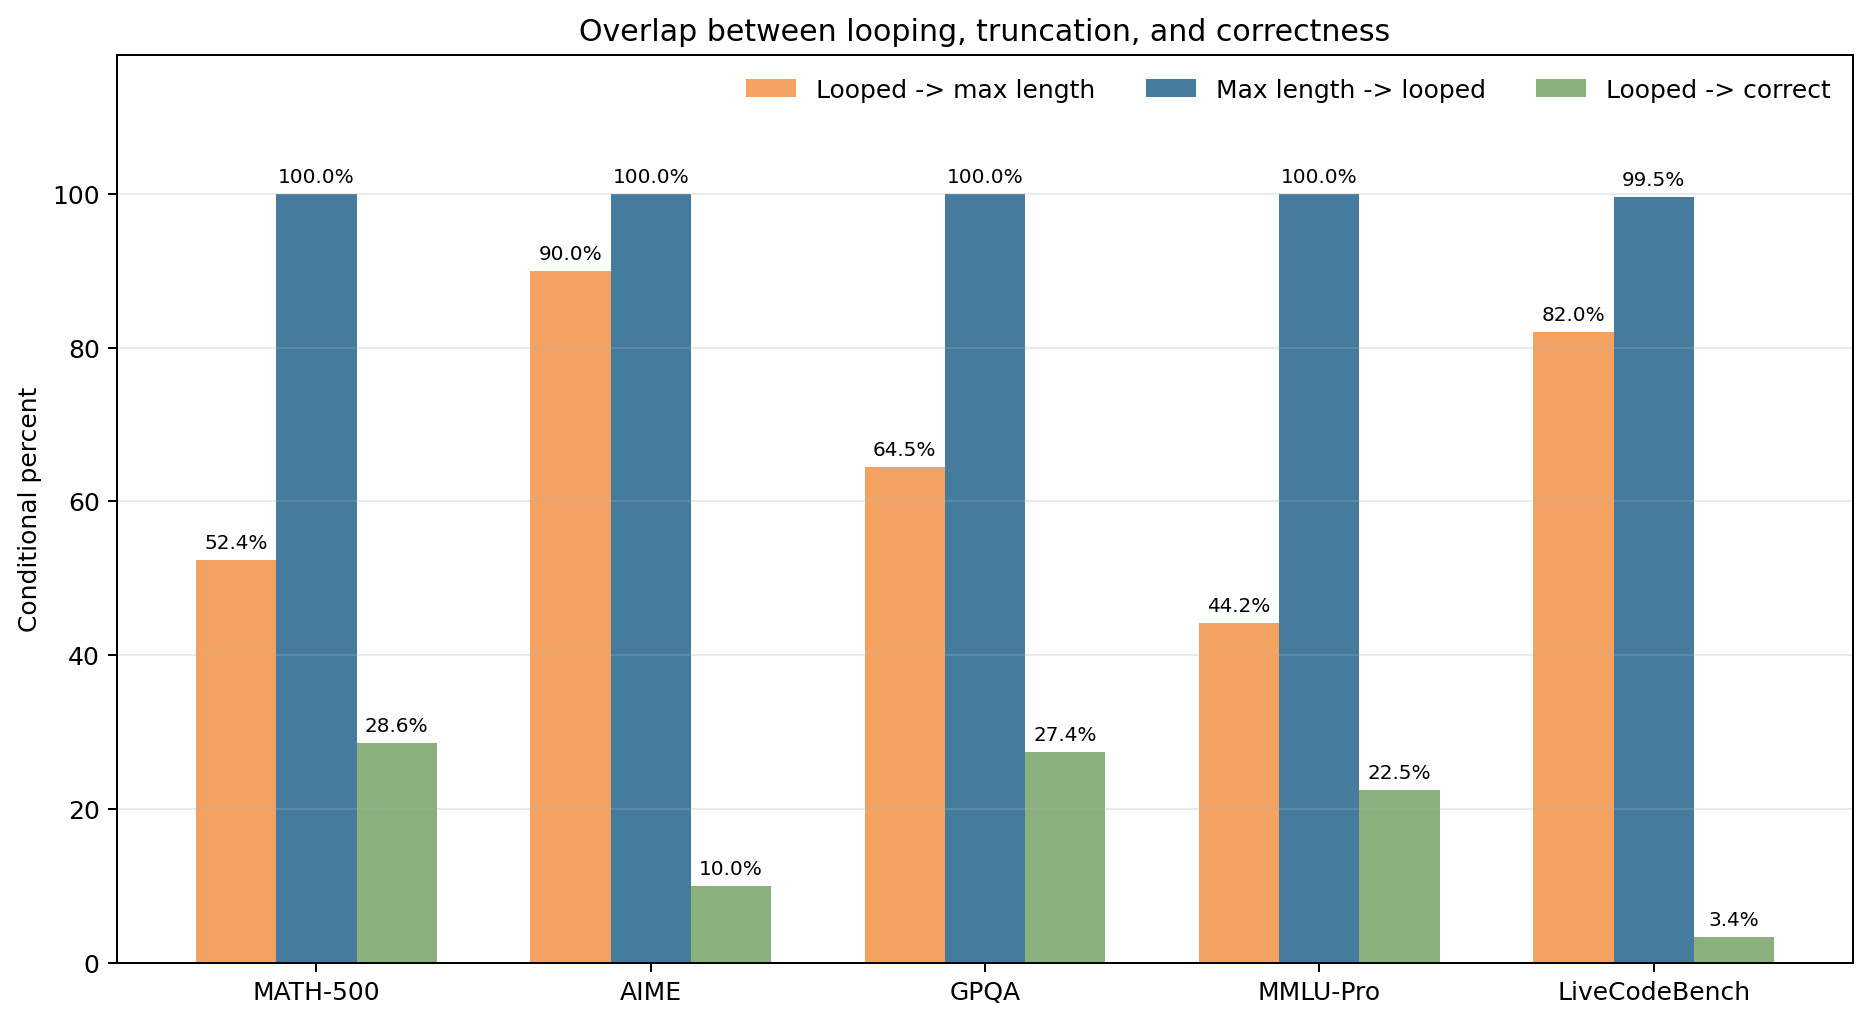
\includegraphics[width=\textwidth]{figures/cross_dataset_overlap.png}
\caption{Overlap statistics: among looped rollouts, how many hit max model length; among max-length-hit rollouts, how many looped; and among looped rollouts, how many still answered correctly.}
\end{figure}

\begin{figure}[H]
\centering
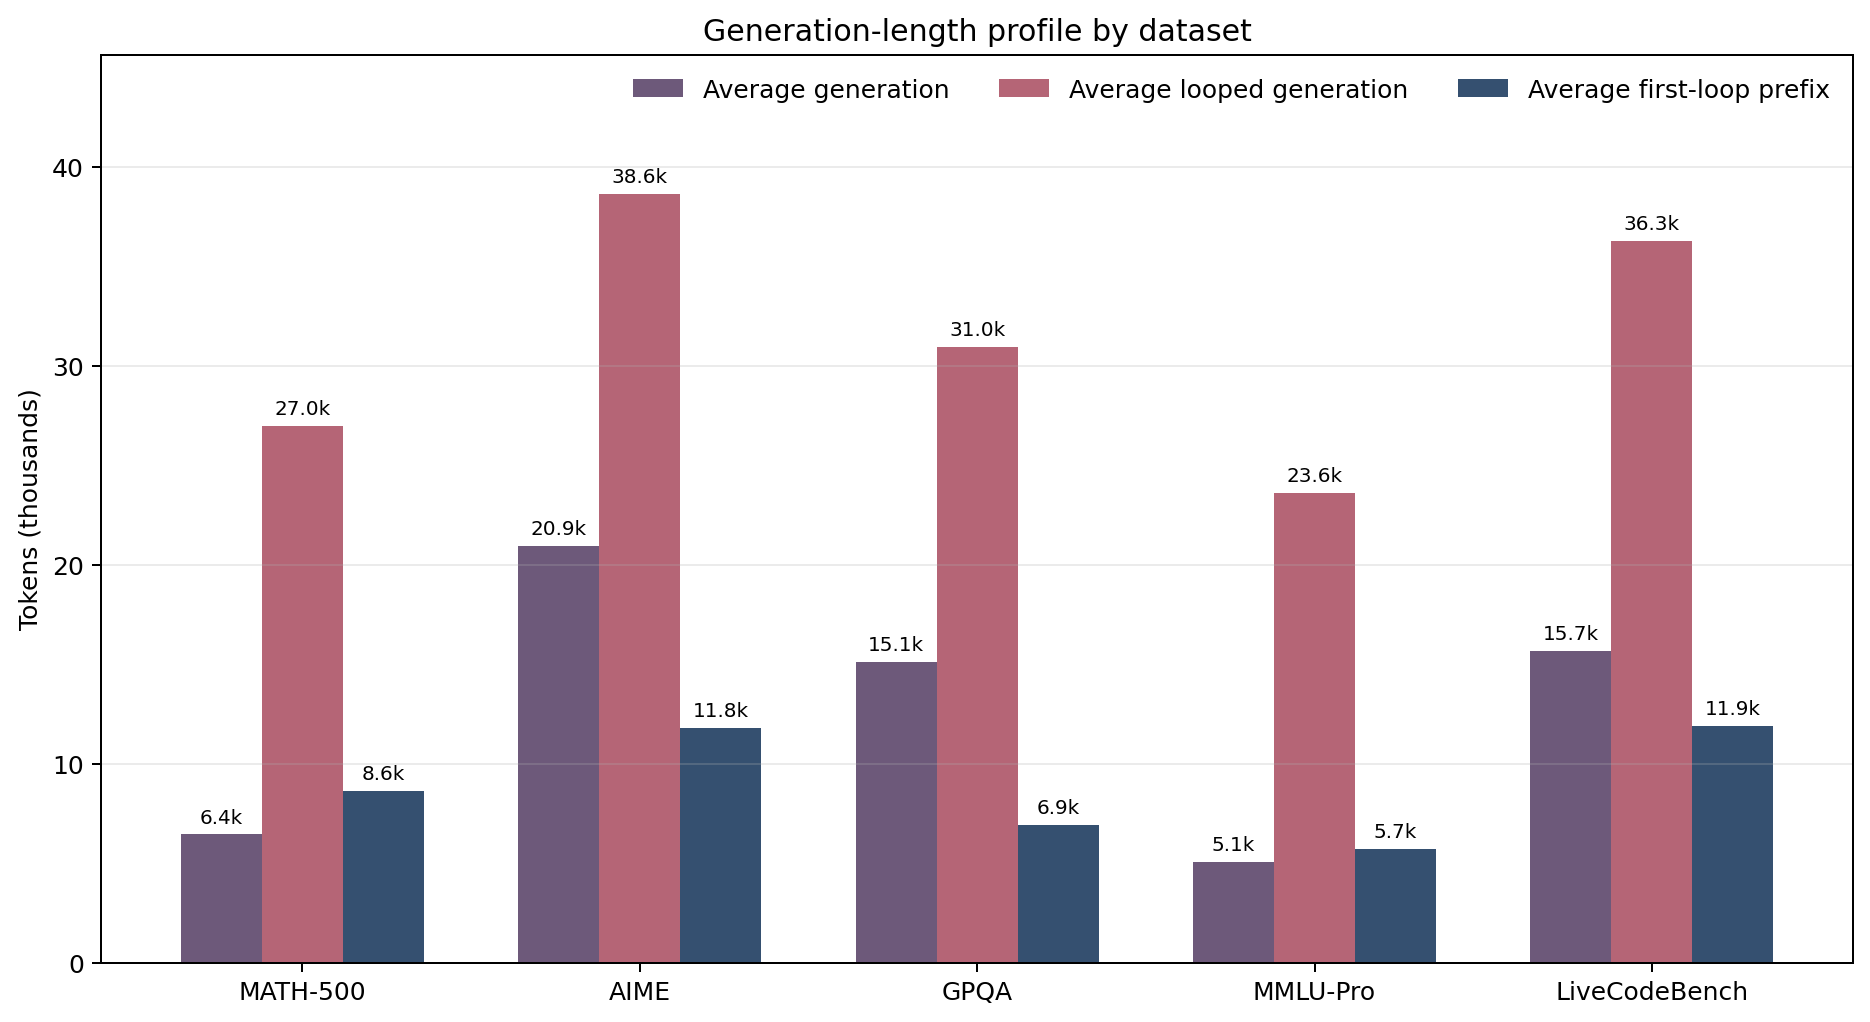
\includegraphics[width=\textwidth]{figures/cross_dataset_lengths.png}
\caption{Average generation lengths, average looped-generation lengths, and average first-loop-prefix lengths in thousands of tokens.}
\end{figure}

\section*{Interpretation}
Across the math, science, broad-knowledge, and coding settings, the same pattern repeats: long generation tails are where looping lives. The strongest evidence is in the overlap panel: once a rollout hits max model length, it is almost always also a detected loop, especially on \texttt{GPQA}, \texttt{MMLU-Pro}, and \texttt{LiveCodeBench}. The converse is weaker but still substantial: a large fraction of looped rollouts on the non-math datasets also terminate at the model-length ceiling.

The length panel shows that looped generations are dramatically longer than the dataset-wide average everywhere. That gap is modestly above \texttt{+16k} tokens on \texttt{GPQA} and grows to roughly \texttt{+20k} tokens on both \texttt{MATH-500} and \texttt{LiveCodeBench}. The average first-loop-prefix length also differs by task family: \texttt{GPQA} loops are typically detected earlier than the long-form math and coding loops, while \texttt{AIME} and \texttt{LiveCodeBench} often burn more than \texttt{10k} tokens before the repeated n-gram pattern is first visible.

Correctness under looping is dataset-dependent. \texttt{GPQA} and \texttt{MMLU-Pro} still retain a non-trivial fraction of correct answers inside looped rollouts, which suggests some looping trajectories occur after the model has effectively committed to the right option. \texttt{LiveCodeBench} is qualitatively different: looped rollouts there are rarely correct, so looping aligns more directly with task failure than with benign verbosity.

\end{document}
